\chapter{Johnson-Rauschen}
In diesem Teil des Experiments wird das Johnson- oder thermische Rauschen untersucht. Dieses Rauschen entsteht durch die thermisch bedingte Bewegung freier Elektronen in ohmschen Widerständen. 
Die Bewegung von Elektronen ist aufgrund zufälliger thermischer Energie ungeordnet und wird daher durch die statistische Physik beschrieben. In einem unbelasteten Stromkreis bewegen sich freie Elektronen ohne äußere Einflüsse zufällig, was zu Impulsübertragung und unabhängigen Spannungs- und Stromschwankungen führt. Diese überlagern sich und bilden das sogenannte weiße Rauschen.

Weißes Rauschen zeichnet sich durch eine gleichmäßige Leistungsverteilung über alle Frequenzen aus.
Das Johnson-Rauschen ist ein Sonderfall dieses Phänomens und lässt sich durch die thermische Bewegung von Elektronen in einem Leiter erklären. Die effektive Spannung $\langle V^2 \rangle$, die sich bei einer Temperatur T an einem Widerstand R einstellt, wird durch die Nyquist-Relation \cite{Nyquist} beschrieben:
\begin{equation}
\langle V^2 \rangle = 4 k_B T R \Delta f,
\label{eq:nyquist}
\end{equation}
wobei $k_B$ die Boltzmann-Konstante und $\Delta f$ die betrachtete Frequenzbandbreite darstellt.
%=======================================================================================================
\section{Aufbau}
\FloatBarrier
\begin{figure}[htbp]
    \centering
    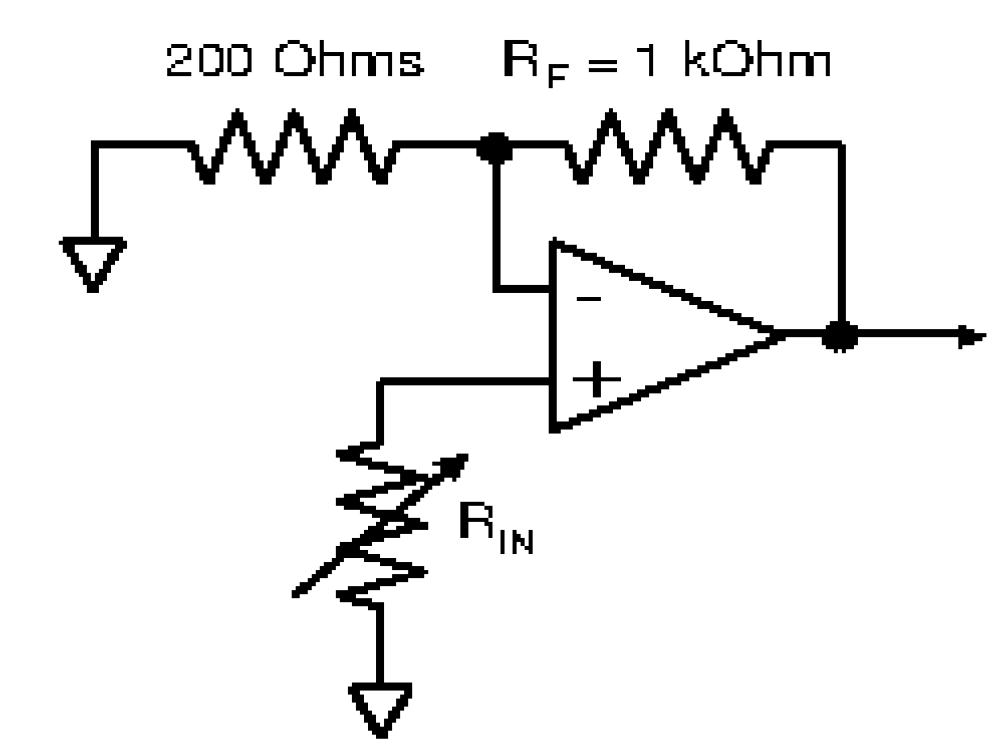
\includegraphics[width=0.5\textwidth]{figs/schalt amplifier.png}
    \caption{Schaltplan des Vorverstärkers der LLE-Box zur Messung des JohnsonRauschens \cite{praktikum}}
    \label{fig:schaltamplifier}
\end{figure}
\FloatBarrier
Da Johnson-Rauschen eine sehr geringe Signalstärke aufweist, ist eine spezielle Verstärkerschaltung erforderlich, um es sichtbar zu machen. Diese ist in Abbildung \ref{fig:schaltamplifier} dargestellt. Es handelt sich um einen nichtinvertierenden Verstärker, integriert in einer sogenannten LLE-Box (Low Level Electronics). Der vollständige Schaltplan ist in Abbildung \ref{fig:johnson lle} dargestellt.
\FloatBarrier
\begin{figure}[htbp]
    \centering
    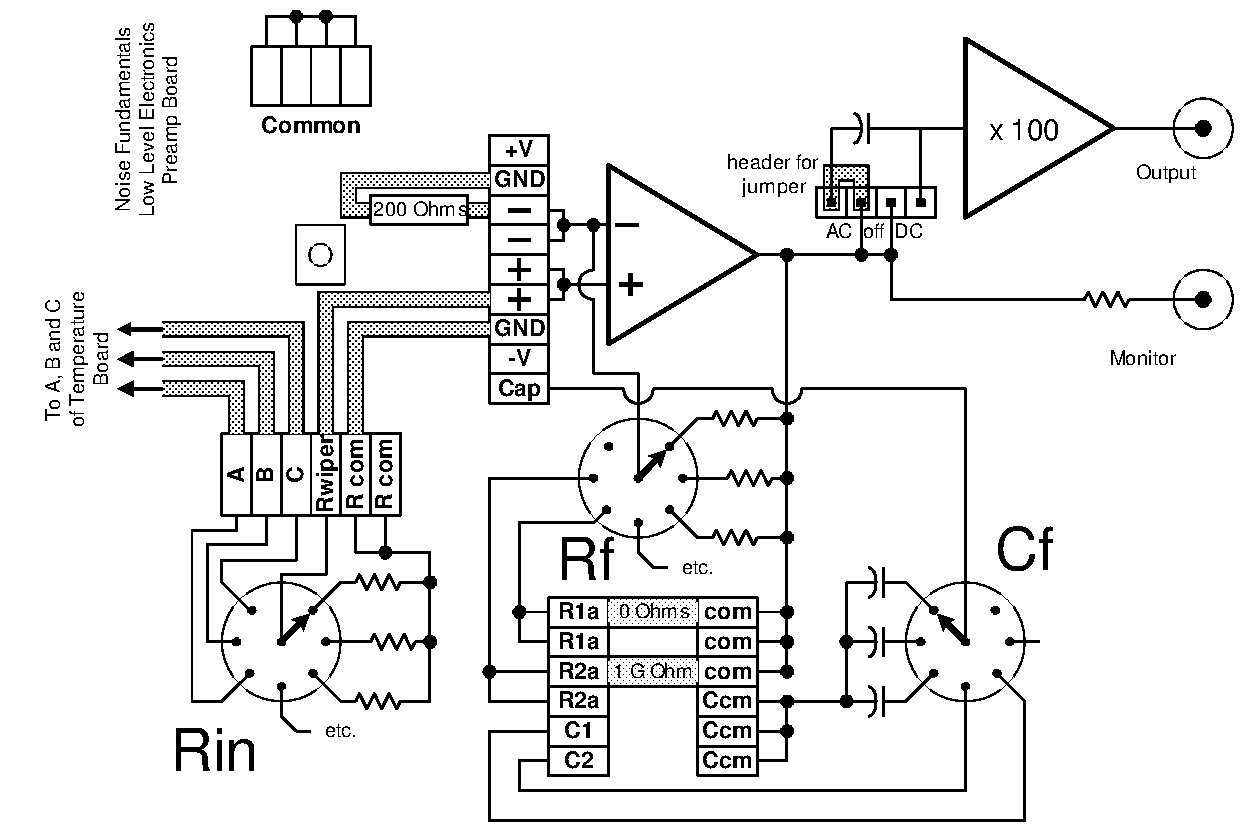
\includegraphics[width=0.75\textwidth]{figs/johnson lle.png}
    \caption{Interner Schaltplan der LLE-Box zur Messung des Johnson-Rauschens \cite{praktikum}}
    \label{fig:johnson lle}
\end{figure}
\FloatBarrier
Nach der Vorverstärkung gelangt das Signal in die HLE-Box (High-Level Electronics, Abbildung \ref{fig:johnson hle}), wo ein Bandpassfilter die relevanten Frequenzbereiche gezielt herausfiltert. Der Ausgang des Vorverstärkers wird dazu über ein BNC-Kabel mit dem Filtereingang der HLE-Box verbunden. Ein zweiter Filter in der HLE-Box ermöglicht die Implementierung eines zusätzlichen Bandpassfilters.
\FloatBarrier
\begin{figure}[htbp]
    \centering
    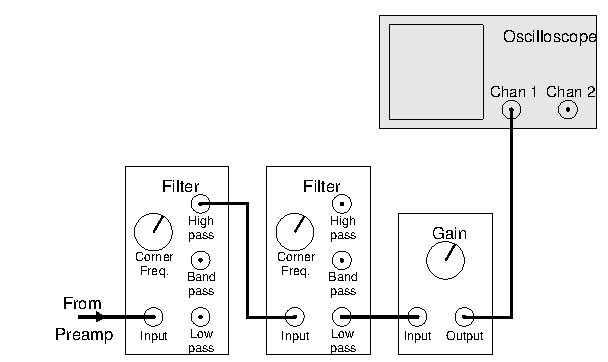
\includegraphics[width=0.5\textwidth]{figs/johnson hle.png}
    \caption{Schaltung der HLE-Box zum Visualisieren des Johnson-Rauschens \cite{praktikum}}
    \label{fig:johnson hle}
\end{figure}
\FloatBarrier
%========================================================================================================
\section{Durchführung und Auswertung}
%---------------------------------------------------------------------------------------------------
\subsection{Beobachten des Johnson-Rauschens}
Die Widerstände der LLE-Box sind auf $R_{in} = 100 k\Omega$  und $R_f = 1 k\Omega$ eingestellt, und die Verstärkung des Signals beträgt G = 600. Das Rauschen wird über einen Oszilloskop-Ausgang mit den Einstellungen $2\,\text{mV/div} \,, \quad 10\,\mu\text{s/div} \,, \quad \text{Triggerlevel} \approx 0$ und einer Eingangsimpedanz von $1\,\text{M}\Omega$ beobachtet. Die Grenzfrequenz des Hochpasses wird auf $f_{gr} = 0,1 kHz$, die Grenzfrequenz des Tiefpasses auf $f_{gr} = 100 kHz$, und der Gain wird auf $G_2 = 300$ eingestellt, um das Johnson-Rauschen zu isolieren. Die Messung erfolgt bei Raumtemperatur, um die thermischen Effekte zu berücksichtigen. Das Rauschen wird in Form eines zeitlichen Verlaufs auf dem Oszilloskop dargestellt, wobei die Amplitude des Rauschens in Millivolt und die Zeit in Mikrosekunden angegeben sind.
 beobachtet. Wenn ein Bandpassfilter mit einer Grenzfrequenz von 10 kHz verwendet wird, ist das Rauschen auf dem Oszilloskop sichtbar. Ohne Filter ist das Rauschen nicht erkennbar, da es von anderen Störsignalen überlagert wird. Die Abbildung \ref{fig:johnson noise} zeigt das Johnson-Rauschen ohne Filter, während Abbildung \ref{fig:bandfilter} das Rauschen mit einem Bandpassfilter darstellt.
 \FloatBarrier
\begin{figure}[htbp]
    \centering
    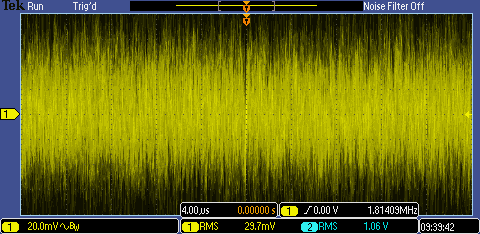
\includegraphics[width=0.5\textwidth]{figs/johnson_noise_without_filter.png}
    \caption{Johnson-Rauschen ohne Filter}
    \label{fig:johnson noise}
\end{figure}
\FloatBarrier

\begin{figure}[htbp]
    \centering
    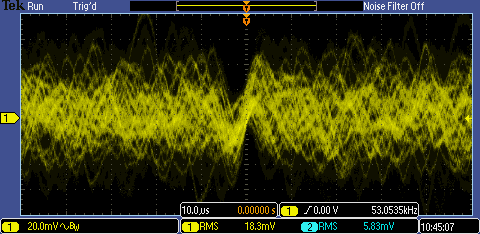
\includegraphics[width=0.5\textwidth]{figs/johnson noise with bandfilter.PNG}
    \caption{Johnson-Rauschen mit Bandpassfilter}
    \label{fig:bandfilter}
\end{figure}
\FloatBarrier

%---------------------------------------------------------------------------------------------------
\subsection{Messung des Johnson-Rauschens}
Zur Messung des Johnson-Rauschens wird ein Widerstand mit einem Wert von 1 k$\Omega$ verwendet. Dieser Widerstand wird in die Schaltung integriert, wie in Abbildung \ref{fig:johnson messung} gezeigt. Der Widerstand ist mit der HLE-Box verbunden, und das Rauschen wird über einen Oszilloskop-Ausgang beobachtet. Die Verstärkung des Signals beträgt G = 600, und die Bandbreite des Filters ist auf 10 kHz eingestellt.
\FloatBarrier
\begin{figure}[htbp]
    \centering
    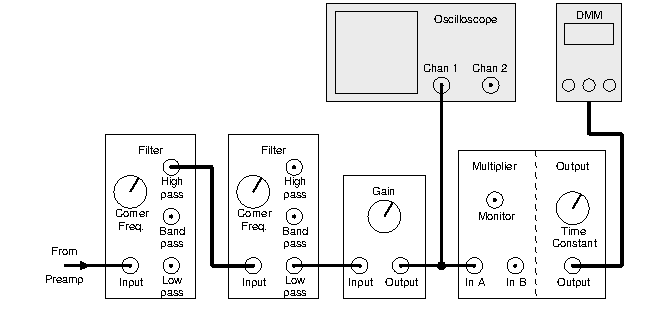
\includegraphics[width=0.5\textwidth]{figs/johnson hle and dmm.png}
    \caption{Verkabelung zur Messung des Johnson-Rauschens \cite{praktikum}}
    \label{fig:johnson messung}
\end{figure}
\FloatBarrier

Um die Funktionalität des Multiplikators zu überprüfen, wird eine Messung durchgeführt, bei der CH1 ,Johnson-Rauschen – $V_{in}$, mit CH2 ,Monitor – Multiplikator – $V_{out}$, verglichen werden. Durch Aktivieren des XY-Modus des Oszilloskops kann die Abhängigkeit der Ausgangsspannung von der Eingangsspannung visualisiert werden. Die resultierende Kurve, dargestellt in Abbildung \ref{fig:parabel}, zeigt einen deutlich erkennbaren, annähernd parabolischen Verlauf. Dies entspricht der theoretisch erwarteten Kennlinie im Verhältnis $V_{out} = (V_{in})^2 / 10 V$, was die korrekte Funktion des Multiplikators empirisch bestätigt. 

\begin{figure}[htbp]
    \centering
    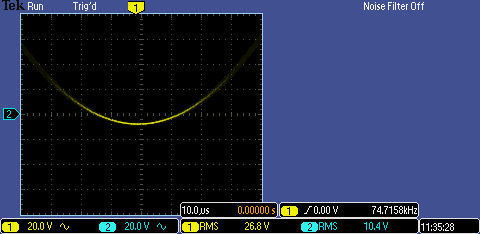
\includegraphics[width=0.5\textwidth]{figs/johnson parabel.png}
    \caption{Darstellung der Abhängigkeit der Ausgangsspannung von der Eingangsspannung im XY-Modus des Oszilloskops}
    \label{fig:parabel}
\end{figure}
\FloatBarrier
%---------------------------------------------------------------------------------------------------
\subsection{Abhängigkeit des Johnson-Rauschens vom Widerstand}
Die Nyquist-Formel postuliert einen linearen Zusammenhang zwischen dem thermischen Rauschen (Johnson-Rauschen) und dem elektrischen Widerstand. Um diesen Zusammenhang experimentell zu überprüfen, wurde die Rauschspannung für verschiedene Widerstandswerte mit einem Digitalmultimeter (DMM) gemessen. Die Widerstände wurden in der LLE-Box auf die Werte 100 $\Omega$, 1 k$\Omega$, 10 k$\Omega$ und 100 k$\Omega$ eingestellt. Die Messung wurde bei konstanter Umgebungstemperatur von $(23,7 ± 0,1) °C$ durchgeführt, um die thermischen Effekte zu berücksichtigen.

Um störende Einflüsse - insbesondere durch das Eigenrauschen nachgeschalteter Verstärkerstufen - zu minimieren, wurde das Verstärkungsverhältnis $G_2$ als fehlerfrei angenommen. Die Unsicherheit der Widerstandswerte wurde mit $1\%$ abgeschätzt, während für die gemessene Spannung eine konstante Unsicherheit von 0,002 V berücksichtigt wurde, um fluktuierende Messabweichungen angemessen zu erfassen.

Es wurde darauf geachtet, dass die resultierende Ausgangsspannung im Bereich von 0.6\,V bis 1.2\,V liegt, da in diesem Bereich eine lineare Proportionalität zur Eingangsspannung gewährleistet ist. Zu diesem Zweck wurde $G_2$ entsprechend angepasst.
Die entsprechenden Messwerte sind in Tabelle \ref{tab:johnson messdaten widerstand} dokumentiert.
\begin{table}[h!]
\centering
\begin{tabular}{|c|c|c|c|c|c|c|c|}
\hline
$R\ (\Omega)$ & $\Delta R\ (\Omega)$ & $U_{\mathrm{DMM}}\ (\mathrm{V})$ & $\Delta U_{\mathrm{DMM}}\ (\mathrm{V})$ & $G$ & $\Delta G$ & $(V_j)^2\ (\mathrm{V}^2)$ & $\Delta (V_j)^2\ (\mathrm{V}^2)$ \\
\hline
1       & 0.01     & 1.000 & 0.002 & 2000 & 0 & $6.94 \times 10^{-12}$  & $1.96 \times 10^{-12}$ \\
10      & 0.1      & 1.002 & 0.002 & 2000 & 0 & $6.96 \times 10^{-12}$  & $1.97 \times 10^{-12}$ \\
100     & 1        & 1.026 & 0.002 & 2000 & 0 & $7.13 \times 10^{-12}$  & $1.99 \times 10^{-12}$ \\
1000    & 10       & 0.713 & 0.002 & 1500 & 0 & $8.80 \times 10^{-12}$  & $2.55 \times 10^{-12}$ \\
10000   & 100      & 0.923 & 0.002 & 1000 & 0 & $2.56 \times 10^{-11}$  & $5.34 \times 10^{-12}$ \\
100000  & 1000     & 0.853 & 0.002 & 400  & 0 & $1.48 \times 10^{-10}$  & $2.03 \times 10^{-11}$ \\
1000000 & 10000    & 0.924 & 0.002 & 300  & 0 & $2.85 \times 10^{-10}$  & $3.25 \times 10^{-11}$ \\
\hline
\end{tabular}
\caption{Gerundete Messdaten zur Bestimmung der thermischen Rauschleistung in Abhängigkeit des Widerstands}
\label{tab:johnson messdaten widerstand}
\end{table}

Der vom Multimeter ausgegebene Messwert hängt in der Folge auf definierte Weise vom quadratischen Mittelwert des Johnson-Rauschens ab:
\begin{equation}
V_{\mathrm{DMM}} = \frac{\overline{V_J^2} \cdot (600 \cdot G_2)^2}{10\,\mathrm{V}}
\label{eq:vdmm}
\end{equation}

Um zusätzliche Rauschkomponenten zu isolieren, die nicht als klassisches Johnson-Rauschen betrachtet werden können, und unter der Annahme, dass Gleichung \ref{eq:vdmm} zusätzliche Störkomponenten enthält ($V_J = V_J^* + V_{\text{Noise}}$), können die vom DMM aufgezeichneten Spannungswerte in die folgende erweiterte Beziehung eingeordnet werden:
\begin{equation}
V_{\mathrm{DMM}} = \frac{(V_J)^2 \cdot (600 \cdot G_2)^2}{10\,\mathrm{V}} = \frac{(V_{J^*} + V_{\mathrm{Noise}})^2 \cdot (600 \cdot G_2)^2}{10\,\mathrm{V}}
\end{equation}

Es folgt: 
\begin{equation}
(V_J)^2 = (V_J^* + V_{\text{Noise}})^2 = V_{J^*}^2 + V_{\text{Noise}}^2 
\end{equation}

Man erhält also folgende lineare Beziehung:
\begin{equation}
        (V_J(R))^2 = \frac{V_{\mathrm{DMM}} \cdot 10\,\mathrm{V}}{(600 \cdot G_2)^2} = V_{J^*}^2 + V_{\text{Noise}}^2 = 4k_B T R \Delta f + V_{\text{Noise}}^2
\end{equation}

Die Messdaten werden im Folgenden mithilfe einer linearen Kleinstquadrate-Anpassung analysiert. Das mittlere quadratische Rauschen wird als Funktion des Widerstands dargestellt.

Dieser Ansatz ermöglicht die Identifizierung der quellenunabhängigen Rauschanteile - insbesondere derjenigen, die nicht vom Widerstand abhängen - als kontinuierliche Verschiebung in Form eines Achsenabschnitts. Das eigentliche Johnson-Rauschen wiederum erscheint als lineare Beziehung zum Widerstand, wie in Gleichung \ref{eq:niquist} theoretisch beschrieben.

Zu diesem Zweck wird eine Regressionsfunktion der Form
\begin{equation}
f(R) = a \cdot R + b
\end{equation}
verwendet, wobei $a$ die Steigung der Geraden und $b$ den Achsenabschnitt repräsentiert und an die Messpunkte aus Tabelle \ref{tab:johnson messdaten Widerstand} angepasst. Die vollständige Darstellung aller Messpunkte ist in Abbildung \ref{fig:fit1} ersichtlich.
\begin{figure}[htbp]
    \centering
    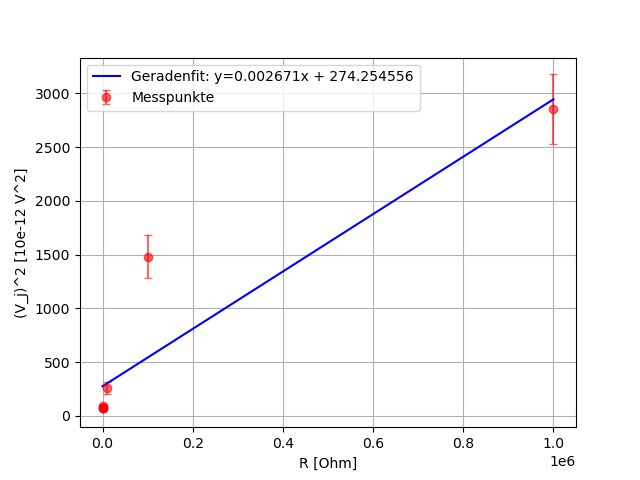
\includegraphics[width=0.5\textwidth]{figs/johnson_resistance.png}
    \caption{Graphische Darstellung der Messdaten und der Regressionsfunktion zur Bestimmung des Johnson-Rauschens in Abhängigkeit des Widerstands}
    \label{fig:fit1}
\end{figure}
\FloatBarrier

Es ergibt sich als Parameter für die Anpassung:
\begin{equation}
a = (2.67 \pm 0.71) \cdot 10^{-3} \, \mathrm{V}^2/\Omega\\
b = (274,25 \pm 12,85) \, \mathrm{V}^2
\end{equation}
%add discussion

Die Steigung $a$ entspricht dem Produkt $4 k_B T \Delta f$, wobei die Temperatur $T$ bei $(23,7 \pm 0,1) °C$ liegt und die Bandbreite $\Delta f = 10\,\mathrm{kHz}$ beträgt. Die Boltzmann-Konstante $k_B$ kann aus der Steigung berechnet werden:
\begin{equation}
k_B = \frac{a}{4 T \Delta f} = \frac{(2.67 \pm 0.71) \cdot 10^{-3} \,\mathrm{V}^2/\Omega}{4 \cdot (23,7 \pm 0,1) \cdot 10^{-3} \,\mathrm{K} \cdot 10 \cdot 10^3 \,\mathrm{Hz}} = (1.38 \pm 0.37) \cdot 10^{-23} \,\mathrm{J/K}
\end{equation}
Dieser Wert liegt im Bereich der allgemein akzeptierten Boltzmann-Konstante von $k_B = 1.38 \cdot 10^{-23} \,\mathrm{J/K}$ \cite{} %add source
, was die Korrektheit der experimentellen Durchführung und der Datenanalyse bestätigt.
%---------------------------------------------------------------------------------------------------
\subsection{Abhängigkeit des Johnson-Rauschens von der Bandbreite}

Die Nyquist-Formel beschreibt eine lineare Abhängigkeit der Rauschleistung von der vom System übertragenen Bandbreite. Zur experimentellen Validierung dieser Beziehung wurden insbesondere im HLE-Gehäuse verschiedene Hochpass- und Tiefpassfilterkonfigurationen implementiert. Um den Einfluss externer Störquellen zu minimieren und thermisches Rauschen zu isolieren, wurde ein Widerstand \(R = 1\,\mathrm{M\Omega} \) verwendet. Aufgrund der direkten Proportionalität des Johnson-Rauschens zum ohmschen Widerstand ist dieser Widerstand hier besonders stark ausgeprägt.

Durch gezielte Variation der Grenzfrequenzen beider Filter konnten unterschiedliche Bandbreiten erreicht werden, deren resultierende effektive Ausgangsspannung mit einem Multimeter aufgezeichnet wurde. Zur anschließenden Analyse wird ein Linearfit erstellt. \\
Dazu wurde die Rausch-Spannung gegen
die Bandbreite aufgetragen. Die Datenpunkte sind in Tabelle Tabelle \ref{tab:gerundet} und das Diagramm in Abbildung \ref{fig:fit2} zu sehen. \\

\begin{minipage}{1.35\textwidth}
%\centering
\begin{adjustbox}{width=0.9\textwidth}
\begin{tabular}{|c|c|c|c|c|c|c|c|c|c|c|c|}
\hline
$f_h$ & $\Delta f_l$ & $f_l$ & $\Delta f_h$ & $G$ & $\Delta G$ & $U_{\mathrm{DMM}}$ & $\Delta U_{\mathrm{DMM}}$ & $\Delta f$ & $\Delta f_{\text{err}}$ & $(V_j)^2$ & $\Delta (V_j)^2$ \\
\hline
300    & 3.00   & 100000  & 1000.00  & 400   & 4   & 0.860  & 0.002 & 99700  & 1.04$\times10^{3}$ & $1.49\times10^{-10}$ & $2.99\times10^{-12}$ \\
1000   & 10.00  & 100000  & 1000.00  & 400   & 4   & 0.846  & 0.002 & 99000  & 1.41$\times10^{3}$ & $1.47\times10^{-10}$ & $2.96\times10^{-12}$ \\
3000   & 30.00  & 100000  & 1000.00  & 400   & 4   & 0.828  & 0.002 & 97000  & 3.16$\times10^{3}$ & $1.44\times10^{-10}$ & $2.90\times10^{-12}$ \\
3000   & 30.00  & 33000   & 330.00   & 600   & 6   & 0.704  & 0.002 & 30000  & 3.02$\times10^{3}$ & $5.43\times10^{-11}$ & $1.10\times10^{-12}$ \\
3000   & 30.00  & 10000   & 100.00   & 1500  & 15  & 1.066  & 0.002 & 7000   & 3.00$\times10^{3}$ & $1.32\times10^{-11}$ & $2.64\times10^{-13}$ \\
100    & 1.00   & 10000   & 100.00   & 1000  & 10  & 0.667  & 0.002 & 9000   & 1.41$\times10^{2}$ & $1.85\times10^{-11}$ & $3.75\times10^{-13}$ \\
100    & 1.00   & 3300    & 33.00    & 2000  & 20  & 0.861  & 0.002 & 3200   & 1.05$\times10^{2}$ & $5.98\times10^{-12}$ & $1.20\times10^{-13}$ \\
100    & 1.00   & 1000    & 10.00    & 4000  & 40  & 0.972  & 0.002 & 900    & 1.01$\times10^{2}$ & $1.69\times10^{-12}$ & $3.39\times10^{-14}$ \\
100    & 1.00   & 330     & 3.30     & 8000  & 80  & 1.010  & 0.030 & 230    & 1.00$\times10^{2}$ & $4.38\times10^{-13}$ & $1.57\times10^{-14}$ \\
10     & 0.10   & 330     & 3.30     & 6000  & 60  & 0.710  & 0.030 & 320    & 1.05$\times10^{1}$ & $5.48\times10^{-13}$ & $2.63\times10^{-14}$ \\
\hline
\end{tabular}
\end{adjustbox}
\caption{Experimentelle Messwerte zur Rauschleistungsanalyse bei variierenden Frequenzen, Verstärkungen und Bandbreiten}
\label{tab:gerundet}
\end{minipage}\\ \\

\begin{figure}[htbp]
    \centering
    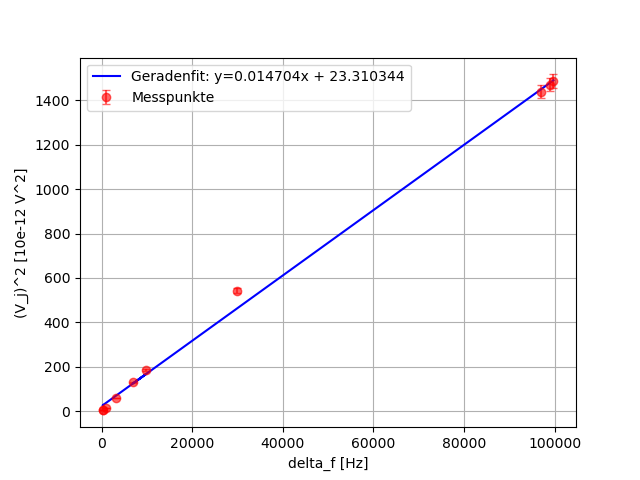
\includegraphics[width=0.5\textwidth]{figs/johnson_bandwith.png}
    \caption{}
    \label{fig:fit2}
\end{figure}
\FloatBarrier
Es ergibt sich als Parameter für die Anpassung:
\begin{equation}
a = (1,47 \pm 0.53) \cdot 10^{-2} \, \mathrm{V}^2/\Omega,   \\
b = (23,31 \pm 2,21) \, \mathrm{V}^2
\end{equation}
Die Steigung $a$ entspricht dem Produkt $4 k_B T \Delta f$, wobei die Temperatur $T$ bei $(23,7 \pm 0,1) °C$ liegt und die Bandbreite $\Delta f$ variiert wurde. Die Boltzmann-Konstante $k_B$ kann aus der Steigung berechnet werden:
\begin{equation}
k_B = \frac{a}{4 T \Delta f} = \frac{(1,47 \pm 0.53) \cdot 10^{-2} \,\mathrm{V}^2/\Omega}{4 \cdot (23,7 \pm 0,1) \cdot 10^{-3} \,\mathrm{K} \cdot \Delta f} = (1,38 \pm 0,49) \cdot 10^{-23} \,\mathrm{J/K}
\end{equation}
Dieser Wert liegt im Bereich der allgemein akzeptierten Boltzmann-Konstante von $k_B = 1.38 \cdot 10^{-23} \,\mathrm{J/K}$ \cite{boltzmann} %add source
, was auf eine sorgfältige Durchführung des Experiments und eine konsistente Datenverarbeitung schließen lässt.
%---------------------------------------------------------------------------------------------------

\end{document}
